\tikzstyle{neuron}=[circle,draw=blue!50,fill=blue!20,thick,minimum size=10mm]
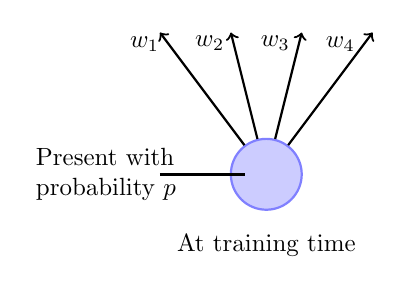
\begin{tikzpicture}[scale=.9, transform shape]
	\node[neuron,minimum width=1 cm] (A) at (2,0) {};
	\draw (0,0) node[text width=2.5cm] {Present with probability $p$};
	\draw[line width=1pt] (0.5,0) -- (1.7,0);
	\draw[thick,->] (A) -- (0.5,2) node[pos=.9,left] {$w_1$};
	\draw[thick,->] (A) -- (1.5,2) node[pos=.9,left] {$w_2$};
	\draw[thick,->] (A) -- (2.5,2) node[pos=.9,left] {$w_3$};
	\draw[thick,->] (A) -- (3.5,2) node[pos=.9,left] {$w_4$};
	\draw (2,-1) node[] {At training time};
\end{tikzpicture}